\documentclass[10pt, a4paper]{article}

\usepackage[english]{babel}
\usepackage{polski}
\usepackage[utf8]{inputenc}
\usepackage{graphicx}
\title{Rozwiązania wybranych zadań z listy nr.1 z przedmiotu "Systemy rozproszone"}
\author{Mateusz Małowiecki}

\begin{document}
\maketitle
\section*{Zad.1 Wiadomo, że pojęcie systemu rozproszonego wymyka się jednej definicji. W praktyce taka standardowa definicja nie jest potrzebna. Istnieją jednak założenia, które są prawdziwe w większością systemów rozproszonych. Spróbuj je wymienić i omówić.}
Pierwszym takim założeniem jest to, że jest on kolekcją kilka komputerów, które działają niezależnie i są w pewien sposób ze sobą powiązane. Drugim założeniem jest to, że użytkownicy myślą, iż pracują na pojedynczym systemie.
\section*{Zad.2 Jaką rolę w systemie rozproszonym odgrywa oprogramowanie warstwy pośredniej?}
Oprogramowanie to ma za zadanie przede wszystkim bycie interfejsem pomiędzy różnymi komputerami oraz zapewnienie systemowi przezroczystości.
\section*{Zad.4 Wyjaśnij, co rozumiemy przez przezroczystość (rozproszenia), i podaj przykłady różnych rodzajów przezroczystości.}
Przezroczystość to ukrywanie różnic między komputerami, sposobów ich komunikacji oraz wewnętrznej organizacji systemu. Rodzaje przezroczystości:
\begin{itemize}
\item{dostępu}
\item{położenia}
\item{wędrówki}
\item{przemieszczania}
\item{zwielokrotnienia}
\item{współbieżności}
\item{awarii}
\item{trwałości}
\end{itemize} 
\section*{Zad.5 Dlaczego czasami tak trudno jest ukryć w systemie rozproszonym występowanie awarii i usuwanie ich skutków (rekonstrukcje, uzdrawianie [systemu], ang. recovery)?}
Awaria może wystąpić w trakcie jakiegoś procesu, w wyniku czego możemy nie mieć możliwości powrotu do stanu sprzed awarii.
\section*{Zad.6 Czy dążenie do osiągnięcia jak największego stopnia przezroczystości jest zawsze dobrym pomysłem? Dlaczego? }
Nie zawsze jest to dobry pomysł. Przykładowo jeśli administrator systemu będzie chciał ukryć awarię pojedynczego komputera w systemie, to może to doprowadzić do awarii całego systemu.
\section*{Zad.7 Co się rozumie przez systemy otwarte? Czy to jest to samo co systemy o otwartym kodzie? Co to jest otwarty system rozproszony i jakie korzyści wynikają z otwartości?}
System otwarty to system, który ma interakcję ze światem zewnętrznym, w szczególności taki system jest przygotowany do komunikacji z każdym innym systemem otwartym. Nie jest to to samo co systemy o otwartym kodzie, ponieważ systemy o otwartym kodzie, to systemy, których kod źródłowy jest publicznie dostępny. Otwarty system rozproszony to zasadniczo system, który oferuje łatwe w obsłudze komponenty mogą być używane lub zintegrowane z innymi systemami.
\section*{Zad.8 Opisz dokładnie, co rozumiemy przez system skalowalny. Scharakteryzuj rodzaje skalowalności.}
Skalowalność oznacza możliwość dodania nowych zasobów i użytkowników, rozmieszczenia węzłów w różnych miejscach. Rodzaje skalowalności:
\begin{itemize}
\item rozmiaru
\item geograficzna
\item administracyjna
\end{itemize}
\section*{Zad.9 Skalowalność można osiągnąć różnymi sposobami. Jakie to są sposoby?}
Te sposoby to:
\begin{itemize}
\item zwiększenie odporności na awarie
\item spójność danych
\item komunikacja asynchroniczna 
\end{itemize}
\section*{Zad.10 Czy wieloprocesory z pamięcią dzieloną są systemami rozproszonymi?}
Tak
\section*{Zad.11 Wieloprocesor z 256 jednostkami centralnymi jest zorganizowany w układzie kraty o wymiarach 16 na 16. Ile wynosi najgorsze opóźnienie (w przeskokach), na jakie jest narażony komunikat}
Najgorsze opóźnienie wynosi 31 i występuje na przykład jeśli idziemy od lewego dolnego rogu do prawego górnego rogu tak jak na obrazku poniżej.
\begin{figure}[h]
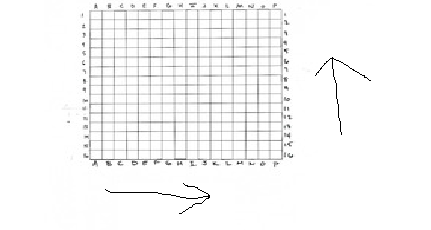
\includegraphics{grid.png}
\end{figure}
\section*{Zad.12 Rozważmy teraz kostkę z 256 jednostkami centralnymi. Ile dla niej wynosi opóźnienie(również w przeskokach) w najgorszym przypadku?}
Opóźnienie dla niej wynosi 8, gdyż odległość między dwoma wierzchołkami tej kostki wynosi co najwyżej 8.
\section*{Zad.13 Na czym polega różnica między rozproszonym systemem operacyjnym a sieciowym systemem operacyjnym?} 
Główna różnica jest taka, że w systemie sieciowym węzły systemu mogą działać na różnych systemach operacyjnych, a w systemie rozproszonym węzły systemu muszą działać na jednym systemie operacyjnym. Więcej o różnicach można przeczytać na stronie: https://www.geeksforgeeks.org/difference-between-network-os-and-distributed-os/.
\section*{Zad.15 Co właściwie oznacza termin "rozproszona pamięć dzielona"?}
Jest to architektura pamięci komputerowej, w której fizycznie oddzielone pamięci mogą być adresowane jako jedna logicznie współdzielona przestrzeń adresowa.
\section*{Zad.17 Czym różnią się systemy zgrupowane (klastrowe) od siatkowych (gridowych)? Jeśli się różnią.}
W systemach zgrupowanych węzły są ściśle połączone za pomocą szybkiej sieci lokalnej. Ponadto na każdym takim węźle działa ten sam system operacyjny. Zupełnie inaczej sytuacja wygląda w przypadku systemów siatkowych. W tym przypadku różne węzły mogą należeć do różnych domen administracyjnych i mogą być bardzo różne pod względem sprzętu, oprogramowania i wdrożonej technologii sieciowej
\section*{Zad.19 Mówi się, że w przypadku zaniechania transakcji świat powraca do poprzedniego stanu,tak jak gdyby transakcja nigdy nie wystąpiła. Nie jest to w pełni prawdziwe. Podaj przykład, w którym odtworzenie poprzedniego stanu świata jest niemożliwe.}
Wyobraźmy sobie, że mamy drukarkę na której coś drukujemy. Gdy w trakcie drukowania strony nastąpi awaria, to nie da się już wrócić do stanu sprzed awarii, ponieważ część kartki jest już zadrukowana.
\section*{Zad.20 Wykonywanie transakcji zagnieżdżonych wymaga jakiejś koordynacji. Wyjaśnij, co faktycznie powinien robić koordynator}
Koordynator powinien koordynować zobowiązania subtransakcji, zgodnie ze standardowym protokołem (zatwierdzeniem rozproszonym).
\section*{Zad.25 Co to jest jednostka centralna (CPU)? Co to jest procesor? Czy terminy CPU i procesor oznaczają to samo?}
Jednostka centralna(CPU) to urządzenie cyfrowe, odpowiedzialne za wykonywanie podstawowych operacji arytmetycznych, logicznych, sterujących oraz operacji wejścia / wyjścia (I / O) określonych przez instrukcje w programie komputerowym. Procesor z kolei jest częścią jednostki centralnej(co w szczególności oznacza, że jednostka centralna może mieć więcej niż jeden procesor).  Widzimy więc, że terminy CPU i procesor nie oznaczają tego samego.
\end{document}